\documentclass[border=2mm]{standalone}
\usepackage{xcolor}
\usepackage{pgfplots}
\usepackage{tikz}
\usetikzlibrary{patterns}

% Define bar chart colors
\definecolor{bblue}{HTML}{4F81BD}
\definecolor{rred}{HTML}{C0504D}
\definecolor{ggreen}{HTML}{9BBB59}
\definecolor{ppurple}{HTML}{9F4C7C}


\begin{document}
	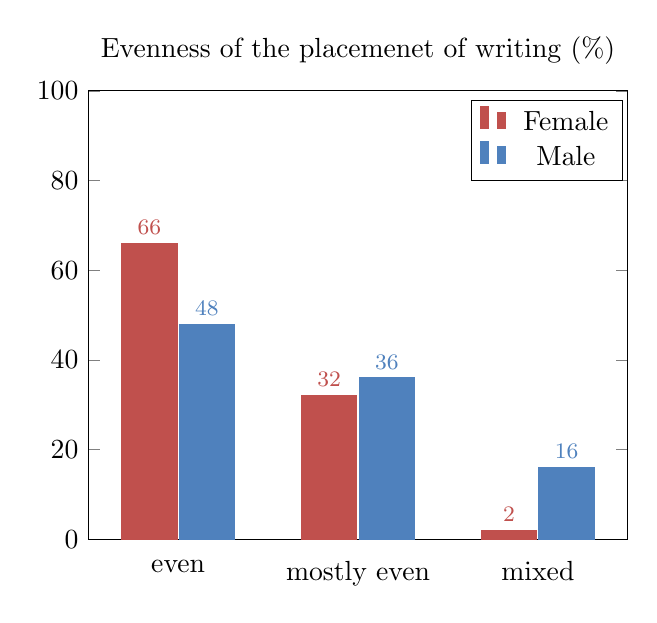
\begin{tikzpicture}
	    \begin{axis}[	
		title={Evenness of the placemenet of writing (\%)},
		major x tick style = transparent,
		%TODO category names
		symbolic x coords={even,mostly even,mixed},		
		xtick = data,
		enlarge x limits=0.25,
		scaled y ticks = false,
		ymin=0,
		ymax=100,
		ybar=2*\pgflinewidth,
		bar width=20pt,
		nodes near coords,
		nodes near coords align={vertical},
		every node near coord/.append style={font=\footnotesize, inner sep=3pt},
		legend cell align=center,
		legend style={
		        at={(0.85,0.98)},
		        anchor=north,
		        column sep=1ex
		}
	    ]

		%TODO category names
		\addplot[fill=rred, rred] coordinates {(even,66) (mostly even,32) (mixed,2)};
		\addplot[fill=bblue, bblue] coordinates {(even,48) (mostly even,36) (mixed,16)};
		
		%TODO group names
		\legend{Female,Male}
	    \end{axis}
	\end{tikzpicture}
\end{document}
